\documentclass[conference]{IEEEtran}
\IEEEoverridecommandlockouts
\usepackage[T1]{fontenc}
\usepackage{cite}
\usepackage{amsmath,amssymb,amsfonts}
\usepackage{graphicx}
\usepackage{booktabs}
\usepackage{xcolor}
\usepackage[hidelinks]{hyperref}
\graphicspath{{figures/}}
\newcommand{\edaN}{200,000}
\newcommand{\edaSignal}{0.530}
\newcommand{\edaDup}{93}
\newcommand{\edaOverlap}{446}


\begin{document}

\title{Expert Features versus Learned Geometry for Higgs Signal Detection:\\
A Calibrated, Statistically Tested Machine-Learning Benchmark\\
\large Phase 1 --- Machine Learning}

% Fill in every team member's name and affiliation before submission.
\author{\IEEEauthorblockN{Ananya Soni}
\IEEEauthorblockA{\textit{Department / Programme} \\
\textit{Institution}\\
City, Country}
}

\maketitle

\begin{abstract}
We classify simulated proton--proton collision events from the UCI HIGGS dataset as a heavy-Higgs
signal or a top-pair background. Following the protocol of Baldi \emph{et al.}, every model is
scored on the same 500{,}000 held-out events, and models are compared at a fixed data budget before
scaling. Phase~1 studies the machine-learning baselines: logistic regression and gradient-boosted
trees (XGBoost) trained on the 21 low-level detector measurements, on the 7 physicist-derived
invariant masses, and on both. We add a physics-motivated feature set built only from the beam's
rotational symmetry (pairwise $|\Delta\phi|$ and $\Delta R$, no masses). Hyperparameters are chosen
by cross-validation on training data only. Probabilities are recalibrated on a dedicated split.
Every AUC carries a DeLong confidence interval, and every claimed difference is a paired DeLong test
repeated over seeds. Results, calibration, compute cost and SHAP-based interpretation are reported in
Sections~\ref{sec:results}--\ref{sec:discussion}.
\end{abstract}

\begin{IEEEkeywords}
Higgs boson, gradient boosting, feature engineering, calibration, DeLong test, SHAP, high-energy physics
\end{IEEEkeywords}

%=====================================================================
\section{Introduction}
High-energy collisions at the Large Hadron Collider (LHC) produce short-lived particles that decay
before reaching the detector; experiments infer what happened from the decay products' momenta,
directions and energy deposits \cite{guest2018deep}. A new particle appears as a small excess of
\emph{signal} events among a much larger \emph{background} of known processes that leave
similar-looking final states. Separating them is a binary classification problem, and the
discovery of the Higgs boson in 2012 \cite{atlas2012observation,cms2012observation} already relied on
multivariate classifiers.

The HIGGS benchmark \cite{baldi2014searching,uci_higgs} isolates this task. Signal is a
hypothetical heavy neutral Higgs boson $H^0$ decaying via $H^0\!\to\!W^\mp H^\pm\!\to\!W^\mp W^\pm h^0\!\to\!W^\mp W^\pm b\bar b$.
Background is top-pair production $t\bar t\!\to\!W^\mp b\,W^\pm\bar b$, which yields the same
visible objects: one charged lepton, missing transverse momentum from a neutrino, and four jets,
some of them $b$-tagged. Each event is described by 21 low-level kinematic features and 7 high-level
invariant masses that physicists designed to reconstruct the intermediate particles.

Baldi \emph{et al.} showed that a deep network trained on the low-level features alone outperformed
shallow models that had the expert features \cite{baldi2014searching}. Phase~1 of this project asks
what \emph{classical} machine learning can do, and why:
\begin{itemize}
\item \textbf{RQ1.} How much do the expert masses help a linear model and a tree ensemble at a fixed budget?
\item \textbf{RQ2.} Can a feature set derived only from a physical symmetry, with no mass
reconstruction, substitute for the expert features?
\item \textbf{RQ3.} What are the calibration and compute trade-offs, and which features do the models use?
\end{itemize}
Our contributions are: (i)~a leakage-controlled, reproducible pipeline with a train/validation/calibration/test protocol;
(ii)~a data-quality audit that ties every exploratory finding to the underlying physics;
(iii)~a rotation-invariant geometric feature set; and (iv)~statistically tested comparisons
(DeLong CIs, paired tests, five seeds) covering discrimination, calibration and cost.

%=====================================================================
\section{Literature Review}\label{sec:lit}
\subsection{Machine learning in high-energy physics}
Multivariate methods, mostly boosted decision trees, have long been standard in collider analyses
\cite{guest2018deep,radovic2018machine}. Baldi \emph{et al.} \cite{baldi2014searching} released the
11M-event HIGGS dataset and reported that boosted trees and shallow networks gain substantially from
the 7 expert features, while a 5-layer network on raw features matched or beat them. The same group
later showed similar gains for $H\!\to\!\tau^+\tau^-$ \cite{baldi2015tautau}. The 2014 Higgs Machine
Learning Challenge \cite{adambourdarios2015higgsml} popularised gradient boosting in the field: XGBoost
was developed and refined there \cite{chen2015higgsboosted}. Later work on jet tagging
\cite{kasieczka2019toptagging,komiske2019energyflow} builds physical symmetries into the
representation. That idea motivates our geometric feature set.

\subsection{Gradient boosting and tabular data}
Gradient boosting fits an additive ensemble of trees by functional gradient descent
\cite{friedman2001greedy}. XGBoost adds a second-order objective, explicit regularisation and a
histogram split finder \cite{chen2016xgboost}; LightGBM offers similar speed-ups \cite{ke2017lightgbm}.
Recent benchmarks find tree ensembles still match or beat deep networks on typical tabular data
\cite{grinsztajn2022tree,shwartzziv2022tabular}. Grinsztajn \emph{et al.} attribute this partly to
trees' robustness to uninformative features and to irregular target functions
\cite{grinsztajn2022tree}. HIGGS is unusual among tabular problems: it is very large and its
features are smooth physical quantities with known symmetries, which is where neural networks are
expected to do well. Random search \cite{bergstra2012random} is an efficient tuning baseline.

\subsection{Evaluation and calibration}
ROC AUC is threshold-free and equals the probability that a random signal event scores above a
random background event \cite{fawcett2006roc}. PR curves are more informative under class imbalance
\cite{saito2015precision}. Models can rank well yet produce miscalibrated probabilities.
Niculescu-Mizil and Caruana showed that boosted trees tend to push probabilities away from 0 and 1,
while logistic regression is often well calibrated \cite{niculescu2005predicting}. Platt scaling
\cite{platt1999probabilistic} and isotonic regression \cite{zadrozny2002transforming} are the
standard post-hoc fixes. All models here share one test set, so their AUC estimates are correlated.
DeLong's non-parametric method \cite{delong1988comparing}, with the fast algorithm of Sun and Xu
\cite{sun2014fast}, gives valid paired comparisons.

\subsection{Interpretability}
SHAP values attribute each prediction additively to the features, with game-theoretic guarantees
\cite{lundberg2017unified}. TreeSHAP computes them exactly and in polynomial time for tree ensembles
\cite{lundberg2020local}.

\subsection{Gap addressed}
Prior HIGGS studies report single-run AUCs without uncertainty, rarely examine calibration, and
compare raw features against expert features without an intermediate representation. We add
seed-repeated, DeLong-tested comparisons, explicit calibration analysis, and a symmetry-derived
middle ground between the two feature sets.

%=====================================================================
\section{Dataset, Quality and Exploratory Analysis}\label{sec:data}
\subsection{Source and protocol}
We use the UCI download \texttt{higgs.zip}. Its single member \texttt{HIGGS.csv.gz} (SHA-256
\texttt{ea302c18\ldots b698}) is streamed and converted once to an $11\text{M}\times29$ float32
memory-mapped array. Following \cite{baldi2014searching}, the last 500{,}000 rows form the test set,
identical for every model and budget. From the remaining 10.5M-row pool we draw a stratified subset
of $N$ events with an explicit seed ($N=250{,}000$ unless stated). The subset is split 80/10/10 into
\emph{train} (fitting), \emph{val} (early stopping only) and \emph{cal} (post-hoc calibration and
stacking only). The label is removed before any transformation, and every transformation is fit on
training rows only.

\subsection{Data quality}
On the \edaN-event training split of seed~0 we find no missing or infinite values and no constant
columns. The signal fraction is \edaSignal, a mild imbalance, which is why PR AUC is reported
alongside accuracy. The UCI file contains exact duplicate events: \edaDup{} repeat within the
training split, none with conflicting labels, and \edaOverlap{} of the 500{,}000 test events also
appear in that training split. This is under 0.1\% of the test set and cannot materially move the
AUCs. We keep the standard test set so results remain comparable with
\cite{baldi2014searching}. The features are pre-standardised in the release (unit variance), so
masses are not in GeV.

\subsection{Physics-grounded checks}
Fig.~\ref{fig:dist} shows class-conditional distributions ordered by single-feature AUC.
Three expectations from the physics are confirmed.
(i)~\emph{Rotational symmetry}: every azimuthal angle $\phi$ is uniform and carries no information
on its own (single-feature AUC $\approx0.500$), because the collision is symmetric about the beam.
(ii)~\emph{$b$-tagging is discrete}: each jet's $b$-tag takes three values.
(iii)~\emph{Mass peaks}: $m_{bb}$, $m_{Wbb}$ and $m_{WWbb}$, the masses of the signal decay chain,
are visibly narrower for signal. $m_{jj}$, $m_{jjj}$, $m_{\ell\nu}$ and $m_{j\ell\nu}$ reconstruct
$W$ and top masses, which the $t\bar t$ background also produces, so they peak for both classes.
Table~\ref{tab:single_auc} shows that no single feature exceeds an AUC of about 0.57, which is why the
problem needs a multivariate classifier. The correlation matrix (Fig.~\ref{fig:corr}) confirms that
the expert masses are non-linear functions of the jet momenta (strongest $|r|\approx0.5$ with jet
$p_T$).

\begin{table}[!t]
\centering
\caption{Most separating single features (training split): ROC AUC of the feature alone.}
\label{tab:single_auc}
\footnotesize
\setlength{\tabcolsep}{3.5pt}
\begin{tabular}{lcc}
\toprule
Feature & Group & AUC \\
\midrule
m\_wwbb & high & 0.575 \\
m\_bb & high & 0.555 \\
missing\_energy\_magnitude & low & 0.543 \\
jet1\_pt & low & 0.538 \\
jet2\_btag & low & 0.527 \\
m\_wbb & high & 0.524 \\
jet4\_pt & low & 0.519 \\
m\_jjj & high & 0.519 \\
\bottomrule
\end{tabular}
\end{table}


\begin{figure*}[!t]
\centering
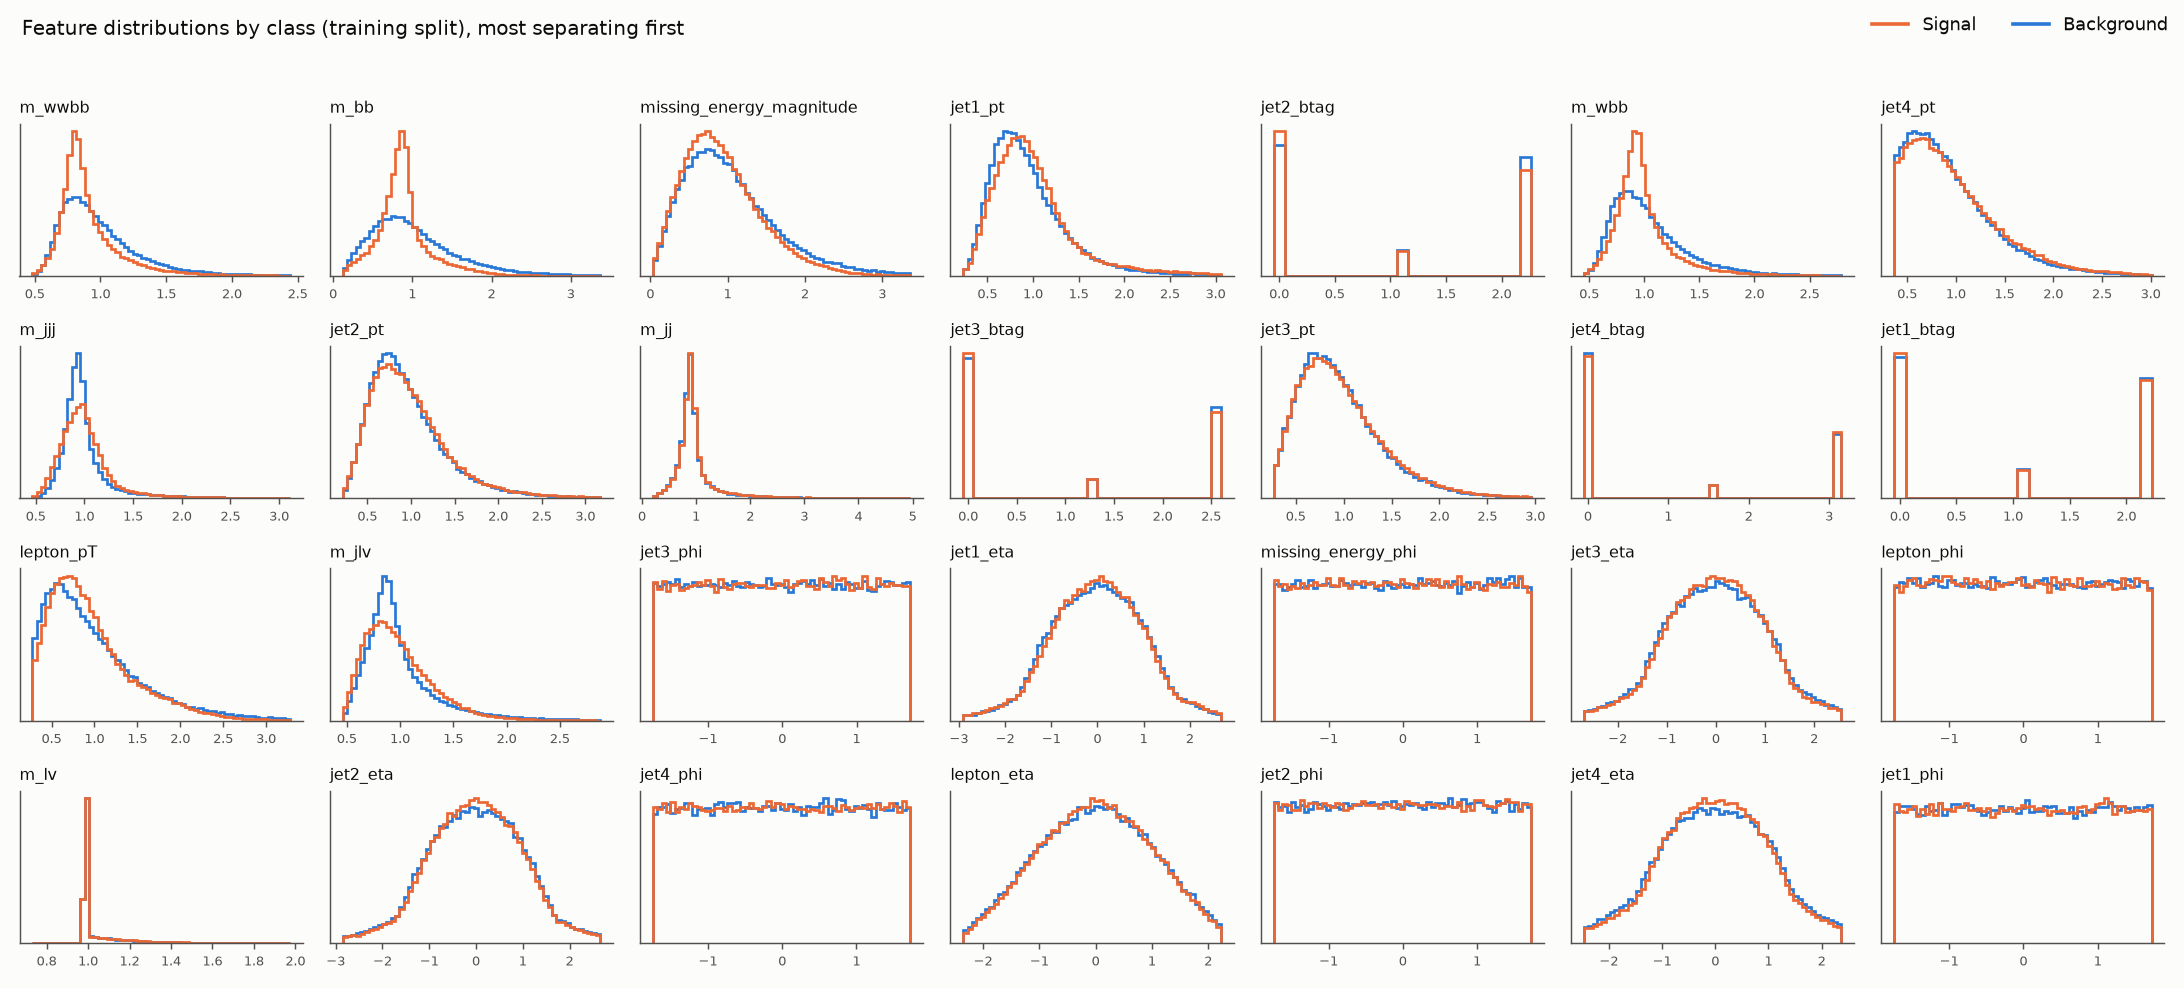
\includegraphics[width=\textwidth]{eda_distributions.png}
\caption{Signal (orange) and background (blue) densities for all 28 features on the training split,
ordered by single-feature AUC. Note the flat $\phi$ distributions, the three-valued $b$-tags, and the
sharper signal peaks of $m_{bb}$, $m_{Wbb}$ and $m_{WWbb}$.}
\label{fig:dist}
\end{figure*}

\begin{figure}[!t]
\centering
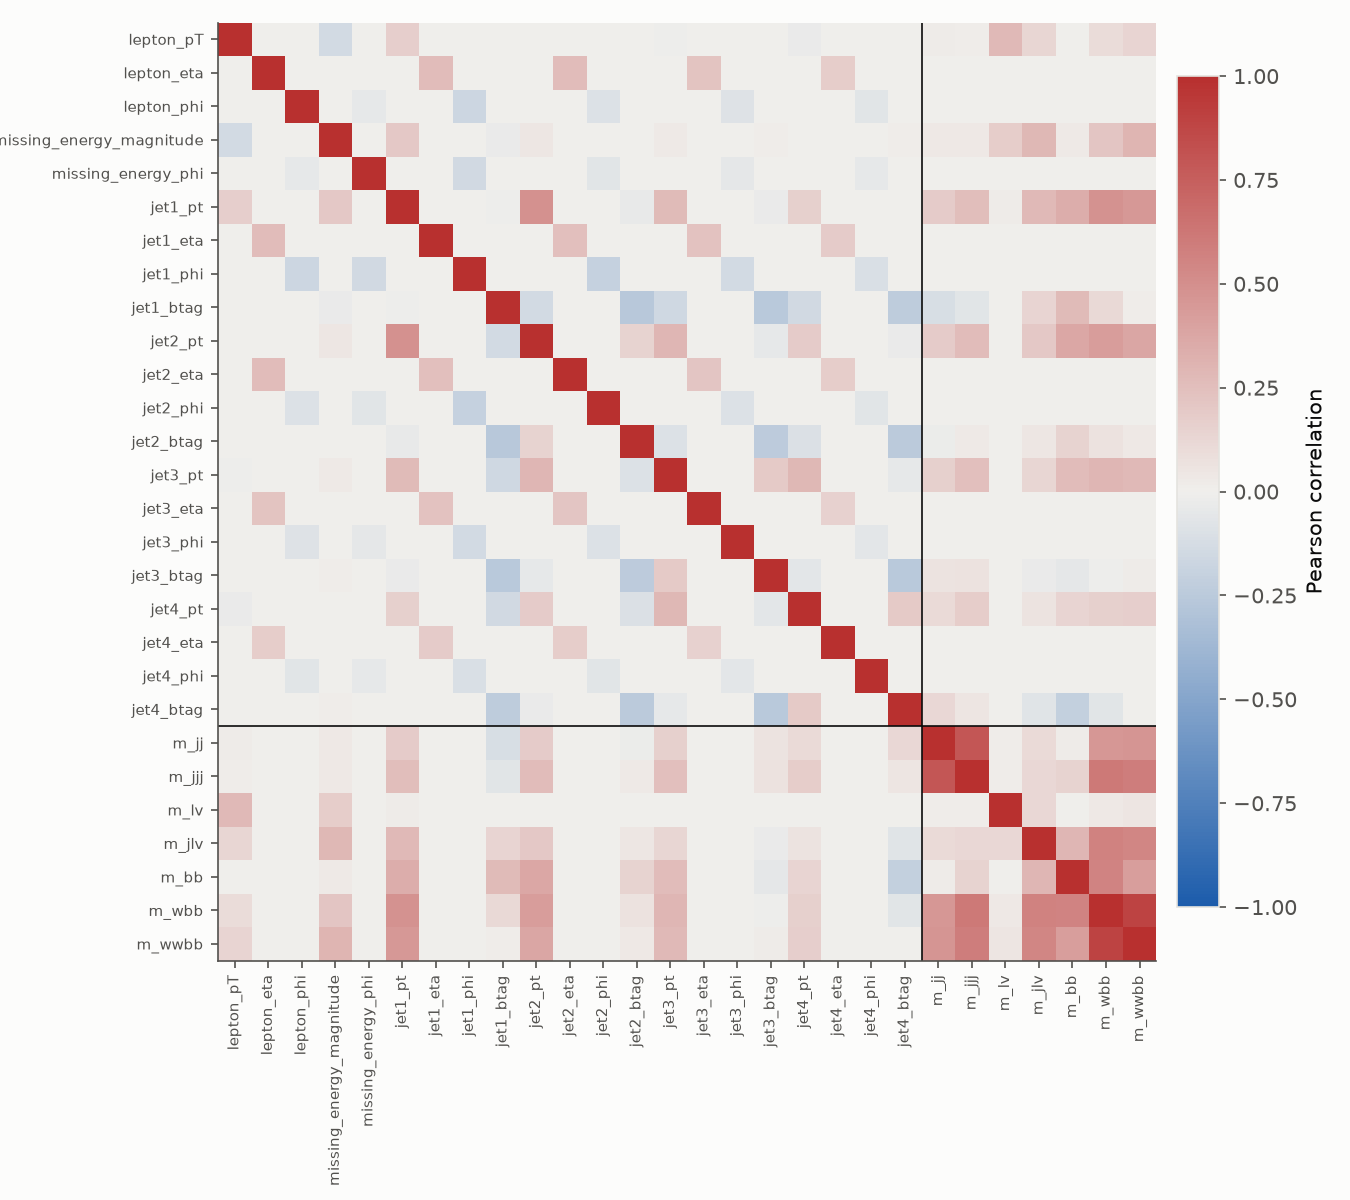
\includegraphics[width=\columnwidth]{eda_correlation.png}
\caption{Pearson correlations. The lines separate low-level (top-left) from expert (bottom-right)
features. The masses correlate with jet $p_T$ but not with any single angle.}
\label{fig:corr}
\end{figure}

%=====================================================================
\section{Feature Engineering}\label{sec:fe}
\subsection{Scaling}
Every feature set is standardised with statistics from the training rows only. Trees are invariant
to this transformation; for logistic regression it makes the L2 penalty treat all features alike.

\subsection{Symmetry-derived geometric features (\texttt{geo})}
The physics of a collision is invariant under a common rotation of every object about the beam axis.
A classifier given absolute angles must learn this invariance from data. We instead re-express
the event in terms that are invariant by construction. The release standardises $\phi$, which is
uniform on $[-\pi,\pi]$, so we recover radians with a factor fit on training rows,
$s=\pi/\max_i|\tilde\phi_i|$, and define for objects $a,b$
\begin{align}
|\Delta\phi_{ab}| &= \bigl|\,((\phi_a-\phi_b+\pi)\bmod 2\pi)-\pi\,\bigr| \in [0,\pi],\\
\Delta R_{ab} &= \sqrt{(\eta_a-\eta_b)^2+\Delta\phi_{ab}^2}.
\end{align}
\texttt{geo} keeps the 15 rotation-invariant low-level features ($p_T$, $\eta$, $|E_T^\mathrm{miss}|$,
$b$-tags), drops the 5 absolute angles, and adds $|\Delta\phi|$ for all 15 pairs of
\{lepton, $E_T^\mathrm{miss}$, jet$_{1..4}$\} and $\Delta R$ for the 10 pairs that have $\eta$:
40 features with no invariant masses. A unit test checks that rotating every $\phi$ in an event by
the same angle leaves all 40 features unchanged. One caveat: $\eta$'s original scale cannot be
recovered from the release, so $\Delta R$ is exact in $\phi$ but approximate in $\eta$.

\subsection{Feature sets compared}
\texttt{low} (21 raw), \texttt{geo} (40), \texttt{high} (7 expert masses), \texttt{all}
(low+high, 28; the set used in \cite{baldi2014searching}), and \texttt{geo+high} (47).

%=====================================================================
\section{Theoretical Background}\label{sec:theory}
\subsection{Logistic regression}
The model is $p(y{=}1\mid\mathbf x)=\sigma(\mathbf w^\top\mathbf x+b)$. It is fit by minimising the
L2-penalised log loss
\begin{equation}
\mathcal L(\mathbf w)=-\sum_i\bigl[y_i\log p_i+(1-y_i)\log(1-p_i)\bigr]+\tfrac{1}{2C}\|\mathbf w\|^2,
\end{equation}
which is convex, so L-BFGS finds the global optimum. The decision boundary is a hyperplane, so the
log-odds must be \emph{linear} in the inputs. That explains its failure on \texttt{low}. The signal
lives in quantities such as $|\phi_a-\phi_b|$ or $\sqrt{(p_a+p_b)^2}$, which are not linear in the
raw coordinates, and a linear function of a uniformly distributed angle cannot express a
dependence on its \emph{difference} with another angle. Giving the model those non-linear quantities
directly (\texttt{geo}, \texttt{high}) is therefore expected to help it most. Because log loss is a
proper scoring rule, the fitted model is close to calibrated whenever it is correctly specified
\cite{niculescu2005predicting}.

\subsection{Gradient-boosted trees}
XGBoost \cite{chen2016xgboost} builds $F_M(\mathbf x)=\sum_{m=1}^M\eta f_m(\mathbf x)$ from
regression trees $f_m$, each fit to a second-order expansion of the loss around the current model.
With gradients $g_i$ and Hessians $h_i$ of the log loss, a leaf $j$ with instance set $I_j$ gets the
optimal weight $w_j^*=-\sum_{I_j}g_i/(\sum_{I_j}h_i+\lambda)$. A split's gain is
\begin{equation}
\tfrac12\!\left[\tfrac{G_L^2}{H_L+\lambda}+\tfrac{G_R^2}{H_R+\lambda}-\tfrac{(G_L+G_R)^2}{H_L+H_R+\lambda}\right]-\gamma,
\end{equation}
where $G,H$ are sums over the left and right children. Trees model interactions up to their depth.
Each split is axis-aligned, however, so a smooth function of a \emph{difference} of two features must be
approximated by a staircase of splits. That is costly in data, which our geometric features remove.
Shrinkage $\eta$, row and column subsampling, $\lambda$, \texttt{min\_child\_weight} and early
stopping on the val split regularise the ensemble.

\subsection{Metrics}
ROC AUC equals the Mann--Whitney statistic
$\hat A=\frac1{mn}\sum_{i\in S}\sum_{j\in B}\mathbb 1[s_i>s_j]$ \cite{fawcett2006roc}. PR AUC (average
precision) emphasises the signal-rich region \cite{saito2015precision}. Log loss and the Brier score
$\frac1n\sum(p_i-y_i)^2$ are proper scoring rules that reward both discrimination and calibration.
Expected calibration error, $\mathrm{ECE}=\sum_b\frac{|B_b|}{n}|\bar y_b-\bar p_b|$ over 15
equal-width bins, isolates calibration.

\subsection{Post-hoc calibration}
Platt scaling fits $\sigma(a\,\mathrm{logit}(p)+c)$ \cite{platt1999probabilistic}. It is monotone, so
AUC is unchanged. Isotonic regression fits any monotone step function \cite{zadrozny2002transforming};
it is more flexible but needs more data. Both are fit on the cal split only.

\subsection{Statistical comparison}
DeLong's estimator \cite{delong1988comparing} writes $\hat A$ as a mean of per-event \emph{placement}
values. This yields the full covariance matrix $\mathbf S$ of $k$ correlated AUCs on the same test
set. A paired test of $A_a=A_b$ uses $z=(\hat A_a-\hat A_b)/\sqrt{S_{aa}+S_{bb}-2S_{ab}}$. We use the
$O(n\log n)$ algorithm of \cite{sun2014fast}, validated against a bootstrap in our tests. Because a
single split can be lucky, every comparison is repeated over five seeds, and we report in how many of
them it is significant.

%=====================================================================
\section{Experimental Setup}\label{sec:setup}
\textbf{Tuning.} On seed~0's training split (test untouched) we run stratified 3-fold CV.
Logistic regression searches $C\in\{10^{-3},\dots,10\}$ (scaler inside the fold). XGBoost runs a
seeded random search of 12 configurations over depth, learning rate, \texttt{min\_child\_weight},
subsampling and $\lambda$, with each fold early-stopped on its own held-out fold. The selection
criterion is mean CV ROC AUC. Table~\ref{tab:tuning} lists the choices, which are then frozen for all
seeds and budgets.

\textbf{Runs.} Five seeds (0--4) at $N=250$k: each seed redraws the subset and reseeds the model. All
models see the same rows within a seed. We then scale to 50k and 1M events (3 seeds each) and to the
full 10.5M pool (1 seed; \texttt{low} and \texttt{all}).

\textbf{Compute.} Python 3.12 with scikit-learn \cite{pedregosa2011scikit} and XGBoost
\cite{chen2016xgboost}, on an Apple M3 with 8\,GB RAM. XGBoost uses all CPU cores with \texttt{hist}
trees.
Reported times are wall-clock training times including early stopping.

\textbf{Reproducibility.} The seed, budget and every hyperparameter live in one \texttt{config.yaml}.
Subset indices and class counts are saved per seed. \texttt{make reproduce} reruns the whole study,
and 12 unit tests (synthetic data, under 10\,s) cover the data splits, feature invariance, metrics,
DeLong, calibration and models.

\begin{table*}[!t]
\centering
\caption{Hyperparameters selected by stratified 3-fold CV on the training split (test untouched).}
\label{tab:tuning}
\footnotesize
\setlength{\tabcolsep}{3.5pt}
\begin{tabular}{lccccccccc}
\toprule
Features & C & CV AUC & depth & $\eta$ & mcw & subs. & colsm. & $\lambda$ & CV AUC \\
\midrule
low (21) & 0.001 & 0.5932 & 10 & 0.05 & 20 & 1 & 1 & 0.1 & 0.7271 \\
geo (40) & 0.01 & 0.6274 & 10 & 0.05 & 20 & 1 & 1 & 0.1 & 0.7918 \\
high (7) & 10 & 0.6455 & 8 & 0.05 & 20 & 0.8 & 1 & 10 & 0.7868 \\
all (28) & 10 & 0.6835 & 8 & 0.05 & 20 & 0.8 & 1 & 10 & 0.8204 \\
geo+high (47) & 10 & 0.6906 & 8 & 0.05 & 20 & 0.8 & 1 & 10 & 0.8340 \\
\bottomrule
\end{tabular}
\end{table*}


%=====================================================================
\section{Results}\label{sec:results}
% Numbers below are copied from results/summary/*.md (generated by scripts/aggregate.py);
% the tables are generated by scripts/make_tables.py.
\begin{table*}[!t]
\centering
\caption{Results at a 250,000-event budget: mean$\pm$sd over 5 seeds, all scored on the same 500k test events. ECE before and after post-hoc calibration on the cal split. Bold: best ROC AUC within the feature set.}
\label{tab:ml_main}
\footnotesize
\setlength{\tabcolsep}{3.5pt}
\begin{tabular}{lcccccccc}
\toprule
Features & Model & ROC AUC & PR AUC & Brier & ECE & ECE$_\mathrm{Platt}$ & ECE$_\mathrm{iso}$ & Train s \\
\midrule
low (21) & LogReg & 0.5957$\pm$0.0001 & 0.6224$\pm$0.0002 & 0.2418$\pm$0.0000 & 0.0155 & 0.0157 & 0.0054 & 0.1 \\
low (21) & XGBoost & \textbf{0.7376$\pm$0.0006} & 0.7481$\pm$0.0006 & 0.2064$\pm$0.0002 & 0.0053 & 0.0058 & 0.0072 & 5.1 \\
geo (40) & LogReg & 0.6298$\pm$0.0001 & 0.6494$\pm$0.0003 & 0.2357$\pm$0.0000 & 0.0079 & 0.0084 & 0.0053 & 0.1 \\
geo (40) & XGBoost & \textbf{0.8011$\pm$0.0005} & 0.8111$\pm$0.0005 & 0.1812$\pm$0.0002 & 0.0037 & 0.0034 & 0.0081 & 11.6 \\
high (7) & LogReg & 0.6450$\pm$0.0004 & 0.6168$\pm$0.0006 & 0.2322$\pm$0.0000 & 0.0480 & 0.0483 & 0.0061 & 0.0 \\
high (7) & XGBoost & \textbf{0.7872$\pm$0.0003} & 0.8050$\pm$0.0003 & 0.1872$\pm$0.0001 & 0.0062 & 0.0051 & 0.0065 & 1.5 \\
all (28) & LogReg & 0.6842$\pm$0.0002 & 0.6828$\pm$0.0003 & 0.2231$\pm$0.0000 & 0.0242 & 0.0246 & 0.0061 & 0.1 \\
all (28) & XGBoost & \textbf{0.8235$\pm$0.0006} & 0.8378$\pm$0.0005 & 0.1711$\pm$0.0003 & 0.0053 & 0.0061 & 0.0067 & 4.8 \\
geo+high (47) & LogReg & 0.6918$\pm$0.0002 & 0.6924$\pm$0.0002 & 0.2206$\pm$0.0000 & 0.0181 & 0.0185 & 0.0064 & 0.2 \\
geo+high (47) & XGBoost & \textbf{0.8381$\pm$0.0003} & 0.8506$\pm$0.0004 & 0.1638$\pm$0.0001 & 0.0054 & 0.0053 & 0.0078 & 10.4 \\
\bottomrule
\end{tabular}
\end{table*}


\subsection{Fixed budget: 250k events, five seeds}
Table~\ref{tab:ml_main} reports every metric as mean$\pm$sd over five seeds. The seed-to-seed sd of
the ROC AUC never exceeds 0.0007, and every difference cited below is significant under the paired
DeLong test in all five seeds ($p<10^{-6}$; Table~\ref{tab:comparisons}).

\begin{table*}[!t]
\centering
\caption{Paired DeLong tests on the shared test set. $\Delta$AUC = A$-$B (mean$\pm$sd over seeds); last column: seeds in which the difference is significant at $\alpha=0.05$ in favour of A / B.}
\label{tab:comparisons}
\footnotesize
\setlength{\tabcolsep}{3.5pt}
\begin{tabular}{lllcc}
\toprule
Question & A & B & $\Delta$AUC & Sig. A/B \\
\midrule
DL vs trees on raw measurements & mlp|low & xgboost|low & 0.0226$\pm$0.0011 & 5/0 \\
DL vs trees on geometric features & mlp|geo & xgboost|geo & 0.0244$\pm$0.0006 & 5/0 \\
DL vs trees on raw + expert & mlp|all & xgboost|all & 0.0075$\pm$0.0005 & 5/0 \\
Feature engineering (geo) for trees & xgboost|geo & xgboost|low & 0.0635$\pm$0.0008 & 5/0 \\
Feature engineering (geo) for the MLP & mlp|geo & mlp|low & 0.0654$\pm$0.0010 & 5/0 \\
Geometry alone vs expert masses (MLP) & mlp|geo & mlp|high & 0.0325$\pm$0.0011 & 5/0 \\
Geometry alone vs expert masses (XGB) & xgboost|geo & xgboost|high & 0.0139$\pm$0.0004 & 5/0 \\
Geometry alone vs raw + expert (MLP) & mlp|geo & mlp|all & -0.0055$\pm$0.0011 & 0/5 \\
geo+expert vs raw+expert (MLP) & mlp|geo\_high & mlp|all & 0.0112$\pm$0.0012 & 5/0 \\
Hybrid 1: wide\&deep vs plain MLP, same inputs & widedeep|geo\_high & mlp|geo\_high & -0.0092$\pm$0.0008 & 0/5 \\
Hybrid 2: stacking vs MLP & stack|geo\_high & mlp|geo\_high & 0.0084$\pm$0.0008 & 5/0 \\
Hybrid 2: stacking vs XGB & stack|geo\_high & xgboost|geo\_high & 0.0124$\pm$0.0001 & 5/0 \\
Hybrid 2: learned stacking vs naive average & stack|geo\_high & average|geo\_high & 0.0002$\pm$0.0000 & 5/0 \\
Hybrid 2 on the paper's features: stacking vs MLP & stack|all & mlp|all & 0.0044$\pm$0.0005 & 5/0 \\
\bottomrule
\end{tabular}
\end{table*}


\textbf{RQ1, value of the expert features.} Logistic regression is close to useless on the raw
measurements (AUC 0.596). The 7 masses lift it to 0.645, and \texttt{all} to 0.684. XGBoost reaches
0.738 on \texttt{low} and 0.787 on \texttt{high}. Combining raw and expert features (\texttt{all},
0.823) adds a further 0.036 over the masses alone. The expert features are therefore worth roughly
0.05--0.09 AUC to both models. Even so, the trees extract substantial information that the masses
do not contain.

\textbf{RQ2, symmetry-derived features.} Replacing the five absolute angles with pairwise
$|\Delta\phi|$ and $\Delta R$ (\texttt{geo}, no masses) raises XGBoost from 0.738 to 0.801
($\Delta=+0.064$). It also lets XGBoost \emph{beat the expert masses} ($+0.014$ over \texttt{high}).
Logistic regression gains $+0.034$ from the same change. Adding the masses to the geometric
features (\texttt{geo+high}) gives the best ML model, XGBoost at 0.838. That is $+0.015$ over the
paper's \texttt{all} feature set. Physical symmetry, with no reconstruction of intermediate
particles, recovers most of what the expert features provide, and it complements them.

\textbf{RQ3, calibration.} XGBoost is well calibrated out of the box (ECE 0.004--0.006), and Platt
scaling leaves it unchanged. Logistic regression shows the opposite failure. Its probabilities are
miscalibrated precisely where the model is misspecified: ECE 0.048 on \texttt{high}, whose masses
relate to the label non-monotonically (Fig.~\ref{fig:shapdep}). Platt scaling cannot fix this
(0.048), because a monotone affine map of the logit cannot change the curve's shape. Isotonic
regression reduces it to 0.006. Fig.~\ref{fig:reliability} shows the reliability diagrams.

\begin{figure*}[!t]
\centering
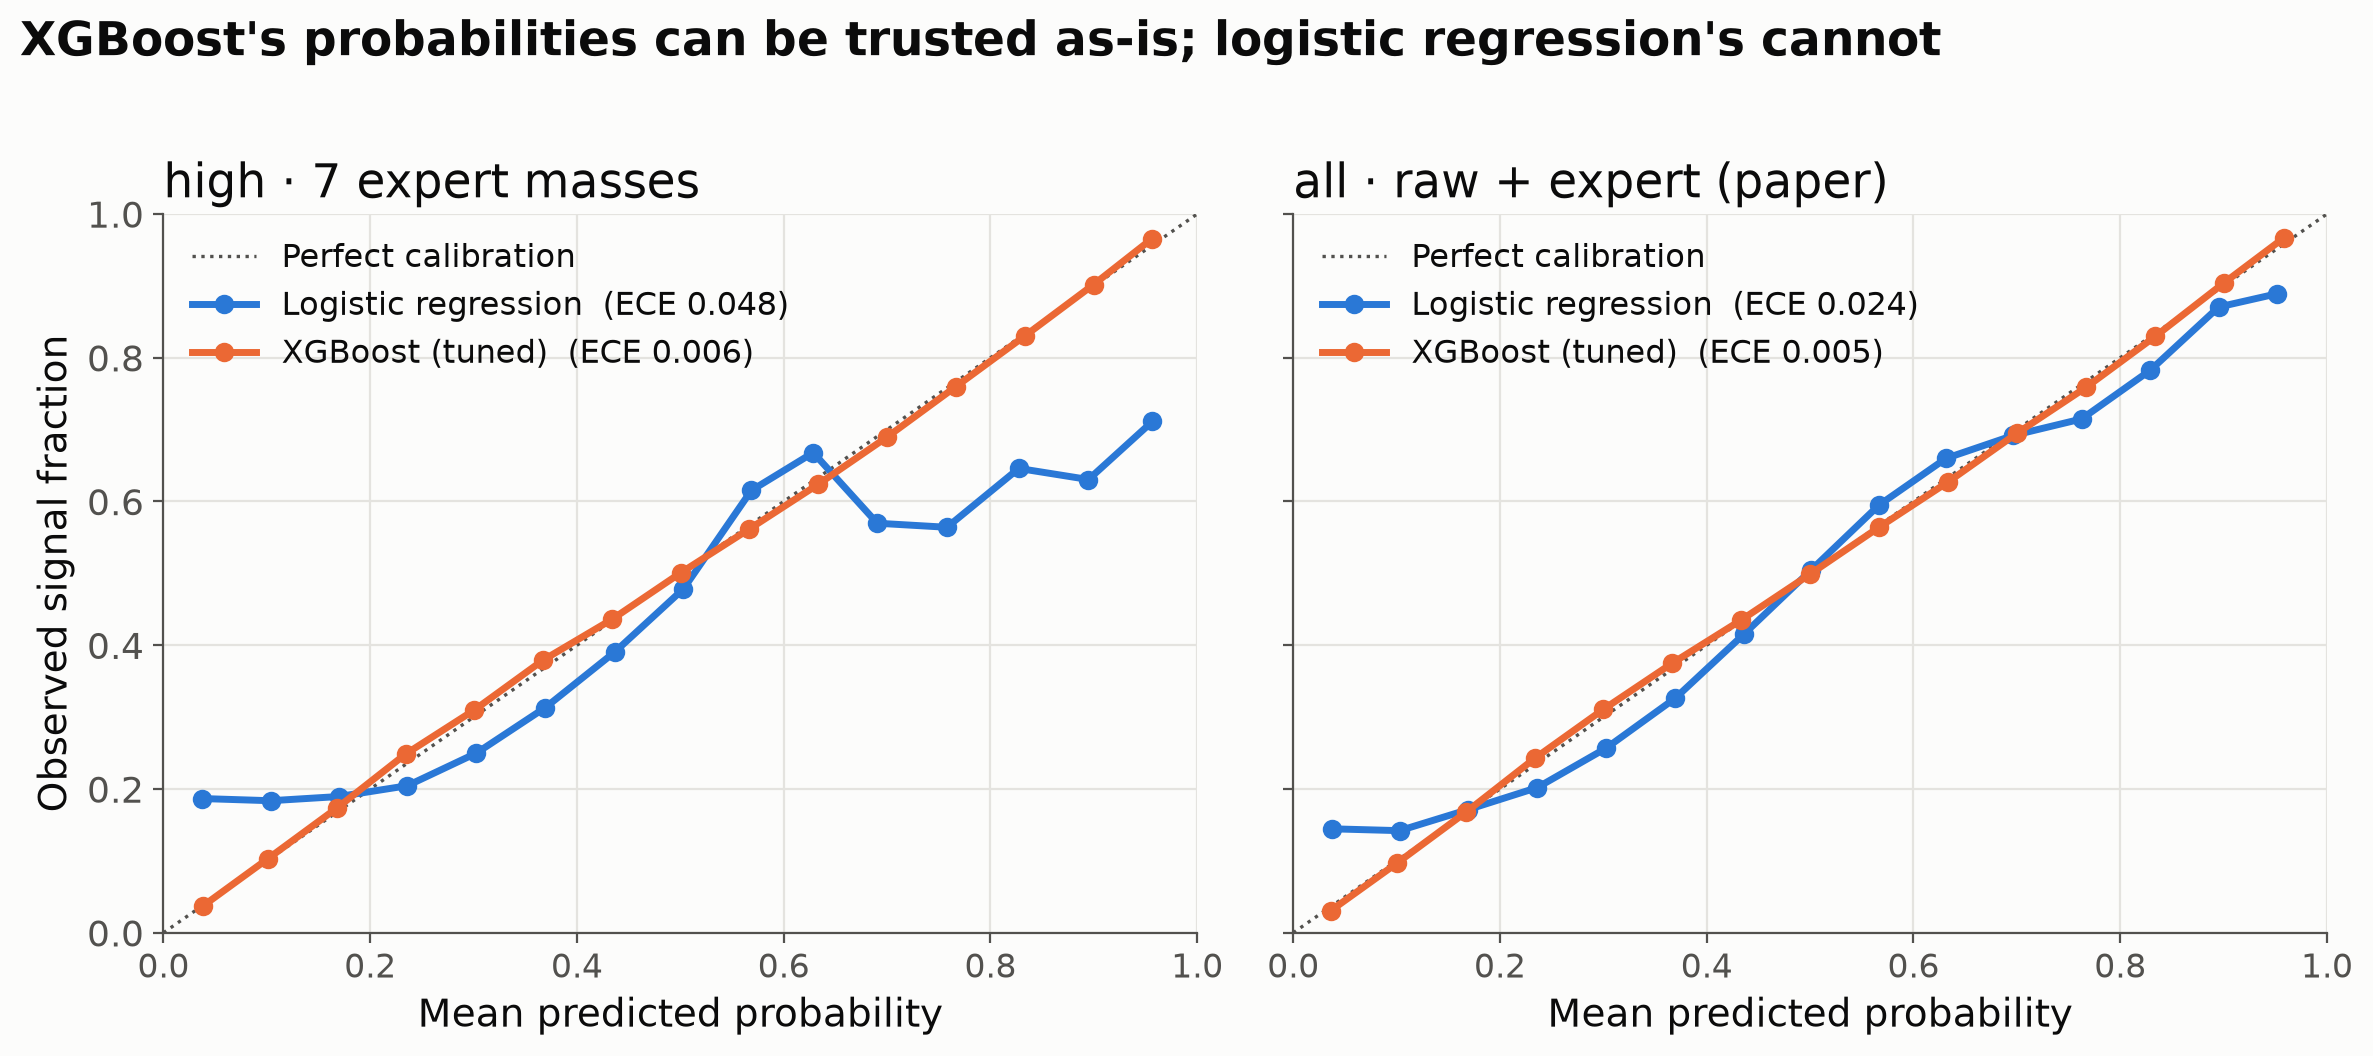
\includegraphics[width=0.85\textwidth]{reliability_ml.png}
\caption{Reliability diagrams on the 500k test events (seed~0, 250k budget, before post-hoc
calibration), for the 7 expert masses (left) and the paper's 28 features (right). XGBoost (orange)
follows the diagonal; logistic regression (blue) bends wherever its linear log-odds are misspecified.}
\label{fig:reliability}
\end{figure*}

\textbf{Compute.} At 250k events, logistic regression trains in under 0.2\,s. Tuned XGBoost needs
1.5\,s (\texttt{high}, 7 features) to 11.6\,s (\texttt{geo}, 40 features, depth 10). The cheapest
strong model is XGBoost on \texttt{all} (4.8\,s, AUC 0.823).

\subsection{Tuning}
Table~\ref{tab:tuning} shows that CV favours deep trees (depth 10 on \texttt{low}/\texttt{geo}, 8
otherwise), a learning rate of 0.05 and a large \texttt{min\_child\_weight} (20). Deep trees are
consistent with the target being a high-order interaction of the raw inputs. Tuning improved
XGBoost by 0.004--0.015 AUC over our initial defaults. For logistic regression the CV AUC varies by
less than $10^{-3}$ across $C$, so the edge-of-grid choices are immaterial.

\subsection{Interpretability}
\begin{table}[!t]
\centering
\caption{Top-10 features of the \texttt{all} set by XGBoost mean $|$SHAP$|$ (log-odds), with logistic-regression $|$coefficients$|$ on standardised inputs.}
\label{tab:importance_ml}
\footnotesize
\setlength{\tabcolsep}{3.5pt}
\begin{tabular}{lcc}
\toprule
Feature & XGB $|$SHAP$|$ & LogReg $|\beta|$ \\
\midrule
m\_bb & 0.635 & 0.600 \\
m\_wwbb & 0.514 & 0.996 \\
m\_wbb & 0.340 & 0.624 \\
m\_jjj & 0.317 & 0.265 \\
m\_jlv & 0.276 & 0.204 \\
jet1\_pt & 0.258 & 0.365 \\
lepton\_pT & 0.172 & 0.171 \\
missing\_energy\_magnitude & 0.134 & 0.238 \\
m\_jj & 0.129 & 0.098 \\
jet2\_pt & 0.102 & 0.087 \\
\bottomrule
\end{tabular}
\end{table}

Both models rank the masses first (Table~\ref{tab:importance_ml}), led by $m_{bb}$ for XGBoost and
$m_{WWbb}$ for logistic regression. The SHAP dependence plots (Fig.~\ref{fig:shapdep}) recover the
physics without being told it. Events whose $m_{bb}$ falls in the peak where $h^0\!\to b\bar b$
decays land are pushed towards signal, by up to $+1$ in log-odds. Events whose three-jet mass
$m_{jjj}$ lies near the top-quark peak are pushed towards \emph{background}, the
$t\!\to\!Wb\!\to\!jjb$ signature. On \texttt{geo}, without masses, XGBoost relies on jet and lepton
$p_T$, the $b$-tags, $|E_T^\mathrm{miss}|$ and the lepton--jet $\Delta R$ values. Those are the
ingredients from which the masses are built.

\begin{figure*}[!t]
\centering
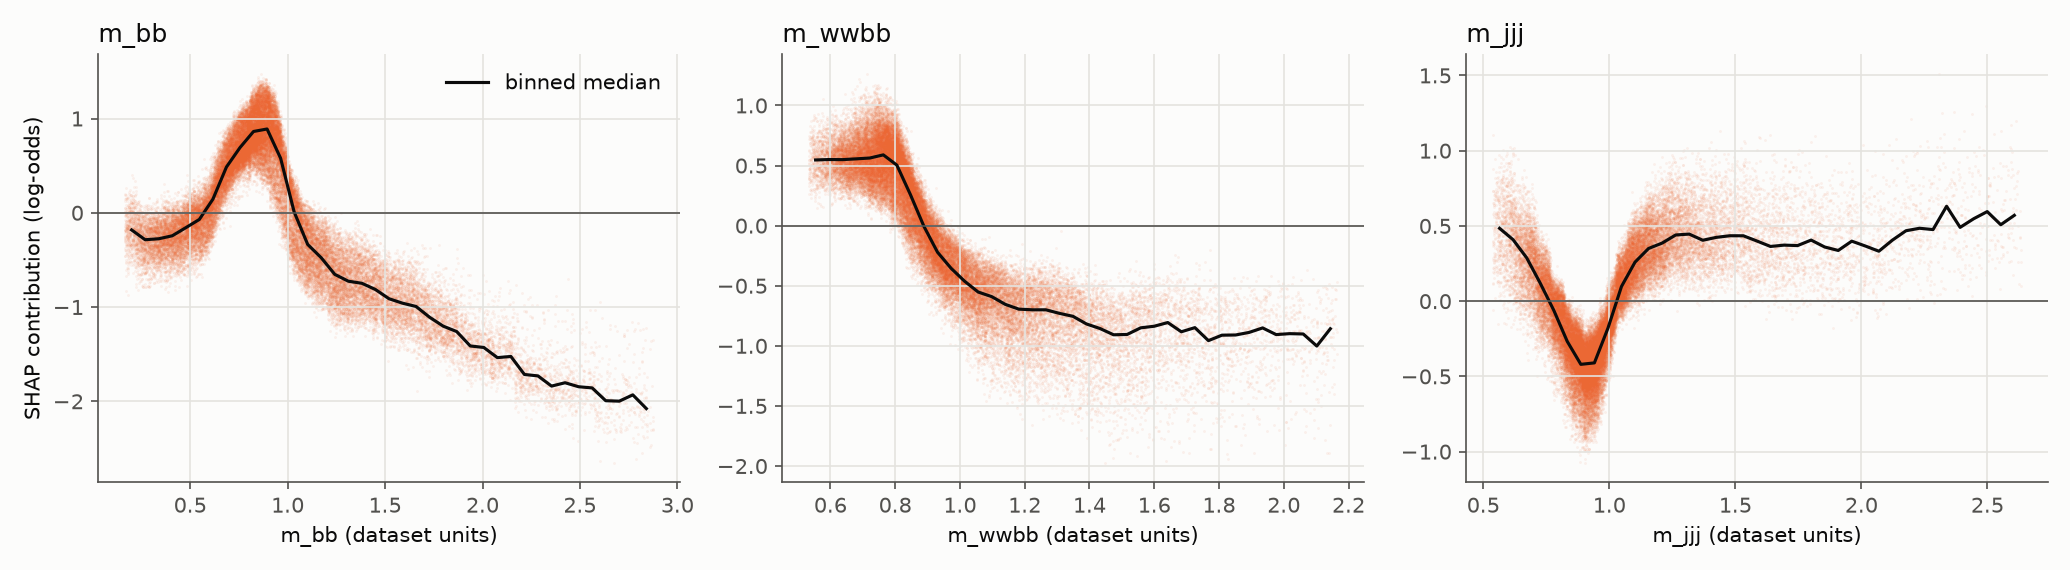
\includegraphics[width=0.92\textwidth]{shap_dependence.png}
\caption{XGBoost TreeSHAP dependence on 50k test events (\texttt{all}, seed~0). Positive values push
towards signal. The $m_{bb}$ peak ($h^0\!\to b\bar b$) favours signal, and the $m_{jjj}$ peak at
the top-quark mass favours the $t\bar t$ background.}
\label{fig:shapdep}
\end{figure*}

\subsection{Scaling beyond the fixed budget}
\begin{table*}[!t]
\centering
\caption{Test ROC AUC vs data budget (train+val+cal events); mean$\pm$sd over seeds (3 seeds; 5 at 250k; 1 at 10.5M, \texttt{low}/\texttt{all} only).}
\label{tab:scaling_ml}
\footnotesize
\setlength{\tabcolsep}{3.5pt}
\begin{tabular}{lccccc}
\toprule
Features & Model & 50k & 250k & 1M & 10.5M \\
\midrule
low (21) & LogReg & 0.5945$\pm$0.0003 & 0.5957$\pm$0.0001 & 0.5959$\pm$0.0000 & 0.5959 \\
low (21) & XGBoost & 0.6986$\pm$0.0011 & 0.7376$\pm$0.0006 & 0.7648$\pm$0.0012 & 0.8001 \\
geo (40) & LogReg & 0.6287$\pm$0.0004 & 0.6298$\pm$0.0001 & 0.6298$\pm$0.0001 & -- \\
geo (40) & XGBoost & 0.7618$\pm$0.0018 & 0.8011$\pm$0.0005 & 0.8230$\pm$0.0005 & -- \\
high (7) & LogReg & 0.6442$\pm$0.0017 & 0.6450$\pm$0.0004 & 0.6450$\pm$0.0003 & -- \\
high (7) & XGBoost & 0.7791$\pm$0.0007 & 0.7872$\pm$0.0003 & 0.7918$\pm$0.0002 & -- \\
all (28) & LogReg & 0.6835$\pm$0.0006 & 0.6842$\pm$0.0002 & 0.6842$\pm$0.0001 & 0.6844 \\
all (28) & XGBoost & 0.8073$\pm$0.0007 & 0.8235$\pm$0.0006 & 0.8365$\pm$0.0001 & 0.8507 \\
geo+high (47) & LogReg & 0.6908$\pm$0.0003 & 0.6918$\pm$0.0002 & 0.6918$\pm$0.0001 & -- \\
geo+high (47) & XGBoost & 0.8180$\pm$0.0005 & 0.8381$\pm$0.0003 & 0.8528$\pm$0.0003 & -- \\
\bottomrule
\end{tabular}
\end{table*}

Table~\ref{tab:scaling_ml} repeats the study at 50k, 1M and the full 10.5M pool. Logistic
regression is flat to within $10^{-3}$ from 50k to 10.5M. It is bias-limited: more data cannot fix a
linear decision boundary. XGBoost keeps improving on every representation, with the largest gains on
raw inputs (\texttt{low}: $0.699\to0.800$). The improvement on the 7 masses saturates quickly
($0.779\to0.792$ from 50k to 1M). At full scale XGBoost reaches 0.851 on \texttt{all}, with the
caveat in Section~\ref{sec:discussion}.


%=====================================================================
\section{Discussion and Limitations}\label{sec:discussion}
\textbf{Why geometry helps trees so much.} A tree can only split on one feature at a time. To use
$\phi_a-\phi_b$, which also wraps at $\pm\pi$, it must tile the $(\phi_a,\phi_b)$ plane with
axis-aligned rectangles. Each rectangle costs data, so the approximation is poor at 200k events.
Supplying $|\Delta\phi|$ and $\Delta R$ turns that staircase into a single split. This is the
mechanism behind the $+0.064$ gain, and it is consistent with Grinsztajn \emph{et al.}'s observation
that trees are sensitive to rotations of the input space \cite{grinsztajn2022tree}. That the gain
exceeds the value of the 7 masses says that much of the information physicists packed into the
masses is angular.

\textbf{Discrimination is not calibration.} XGBoost's log-loss objective and early stopping on log
loss make it well calibrated here. That differs from older findings for boosted stumps
\cite{niculescu2005predicting}. The logistic-regression failure illustrates the general rule that a
proper scoring rule only guarantees calibration for a well-specified model.

\textbf{Statistical versus practical significance.} With 500k test events, DeLong standard errors
are $5$--$8\times10^{-4}$, so differences of 0.002 are already ``significant''. We therefore report
effect sizes, seed-to-seed sd and the number of significant seeds. We only interpret differences
that are consistent across all seeds and at least several times larger than the seed sd.

\textbf{Limitations.}
(i)~The data are simulated and the classes are defined by the generator. High AUC shows separability
of this benchmark, not evidence for the hypothetical particle.
(ii)~The UCI release contains exact duplicate events (\edaOverlap{} test events also appear in a
training split). This is under 0.1\% and immaterial to AUC, but documented.
(iii)~$\Delta R$ is approximate along $\eta$, because $\eta$'s original scale cannot be recovered.
(iv)~Tuning used 12 random configurations on one seed's training split, so a larger search could
add a little.
(v)~At 10.5M events XGBoost reached its 3000-tree cap without early stopping, so that number is a
lower bound.
(vi)~The 1M and 10.5M runs shared an 8\,GB machine and ran under memory pressure, so their wall-clock
times are not used in any compute comparison. All timing claims use the 250k runs.


%=====================================================================
\section{Conclusion}
On a fixed budget of 250k events, tuned XGBoost dominates logistic regression on every
representation. The 7 expert masses are worth 0.05--0.09 AUC. A symmetry-derived representation
built only from pairwise angles and $\Delta R$ outperforms those masses ($+0.014$), and combined
with them gives the best ML model (0.838 vs.\ 0.823 on the paper's feature set). Every one of these
differences holds in all five seeds under paired DeLong tests. XGBoost is well calibrated, while
logistic regression is miscalibrated wherever it is misspecified, which only isotonic recalibration
repairs. SHAP recovers the $h^0\!\to b\bar b$ and top-quark mass peaks unprompted. As data grow
to 10.5M events, the linear model stays flat, while XGBoost keeps improving, fastest on raw inputs.
That trend motivates Phase~2: a model that learns smooth interactions directly may need neither the
masses nor the hand-built geometry.


\bibliographystyle{IEEEtran}
\bibliography{references}
\end{document}
